\newpage
\section{Analisi dei rischi} \label{AnalisiDeiRischi}
	
	Per sviluppare il progetto in maniera efficiente ed efficace viene effettuata un'analisi preliminare dei rischi che possono creare problemi nel processo di sviluppo.
	E' quindi fondamentale avere un sistema che ne permetta la gestione in modo da poter agire immediatamente e con un piano ben definito in caso dovessero presentarsi.
	I seguenti punti rappresentano come il gruppo ha deciso di trattare i rishi:
	
	\begin{itemize}
		\item Identificazione: individuare i potenziali rischi che possono presentarsi
		\item Analisi e valutazione: determinarne la probabilità di occorrenza e comprenderne la criticità
		\item Pianificazione: si definiscono strategie che possono evitare i rischi precendentemente trovati
		\item Controllo: si monitorano e revisionano i rischi finche il progetto procede 
		\item Revisione: in caso dovessero presentarsi rischi (anche imprevisti), dopo averli risolti si rivede la strategia utilizzata e si rivede e migliora in caso qualcosa non ha funzionato come si deve o ci fosse la possibilità
	\end{itemize}
	
	\subsection{Classi di gravità}
	
	Per l'identificazione dei rischi viene utilizzato come strumento di misura la tabella del qualitative risk assessment, in modo da dare a ciascun rischio un valore ben preciso per e catalogarli dal meno al più rischioso.
	
	\begin{center}
		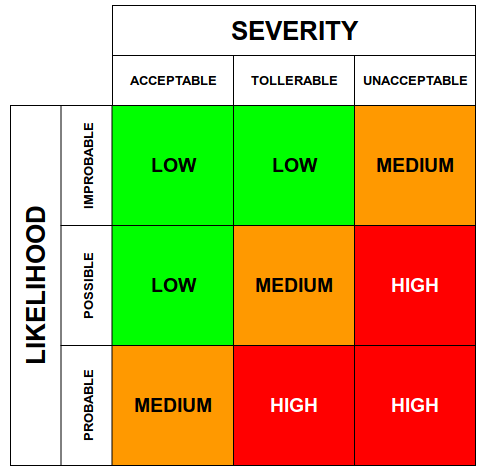
\includegraphics[scale=0.5]{img/tabella.png}
	\end{center}


	I rischi che possono esserci all'interno del progetto rientrano in queste categorie
	
	Di seguito verranno elencati i rischi analizzati dal gruppo nel seguente modo:\\
	
	\begin{table}[H]
		\begin{risktable}{\columnwidth}{m{1.5cm}m{4.1cm}m{4.1cm}m{4.1cm}}
			\thead{ID} & 
			\thead{Probabilità} & 
			\thead{Gravità} & 
			\thead{Classe} \\
			\hline
			\multicolumn{4}{X}{
				\thead{Nome}
			}\\
			\hline
			\multicolumn{4}{X}{
				\thead{Descrizione}
			}\\
			\hline
			\multicolumn{4}{X}{
				\thead{Mitigazione}
			}\\
		\end{risktable}
		\caption{Fac simile tabella rischi}
	\end{table}
	
	Lista rischi possibili: 
	
	\begin{table}[H]
		\begin{risktable}{\columnwidth}{m{1.5cm}m{4.1cm}m{4.1cm}m{4.1cm}}
			ID & 
			Probabilità & 
			Gravità &
			Classe\\
			\hline
			\multicolumn{4}{X}{
				Impreparazione del team a livello tecnico
			}\\
			\hline
			\multicolumn{4}{X}{
				Non tutti i componenti del gruppo hanno le conoscenze di ambienti di sviluppo, linguaggi di programmazione e strumenti richiesti dall'azienda allo stesso livello
			}\\
			\hline
			\multicolumn{4}{X}{
				Le ore di studio peronale si usano per portare il gruppo ad un livello di conoscenza comune
			}\\
		\end{risktable}
	\end{table}

	\mydoublerule{\linewidth}{0pt}{2pt}

	\begin{table}[H]
		\begin{risktable}{\columnwidth}{m{1.5cm}m{4.1cm}m{4.1cm}m{4.1cm}}
			ID & 
			Probabilità & 
			Gravità &
			Classe\\
			\hline
			\multicolumn{4}{X}{
				Impreparazione del team a livello gestionale
			}\\
			\hline
			\multicolumn{4}{X}{
				Non avendo affrontato progetti del genere prima d'ora, i componenti del gruppo non conoscono bene i ruoli che devono intraprendere e i compiti che devono svolgere
			}\\
			\hline
			\multicolumn{4}{X}{
				Durante le ore di studio personale non rendicontate ciascun componente si impegna a studiare la gerarchia dei ruoli fornita nel materiale del professore in modo da essere preparati quando si cambia di ruolo.
				Inoltre, coloro che ricopriranno i ruoli di responsabile e amministratore saranno attenti a controllare che gli altri rispettino i compiti del ruolo a loro assegnato.
			}\\
		\end{risktable}
	\end{table}
	
		\mydoublerule{\linewidth}{0pt}{2pt}
		
\begin{table}[H]
		
		\begin{risktable}{\columnwidth}{m{1.5cm}m{4.1cm}m{4.1cm}m{4.1cm}}
			ID & 
			Probabilità & 
			Gravità &
			Classe\\
			\hline
			\multicolumn{4}{X}{
				Non arrivare giusti ad una scadenza
			}\\
			\hline
			\multicolumn{4}{X}{
				Descrizione
			}\\
			\hline
			\multicolumn{4}{X}{
				Mitigazione
			}\\
		\end{risktable}
	\end{table}
	
	\mydoublerule{\linewidth}{0pt}{2pt}
\begin{table}[H]
		
		\begin{risktable}{\columnwidth}{m{1.5cm}m{4.1cm}m{4.1cm}m{4.1cm}}
			ID & 
			Probabilità & 
			Gravità & 
			Classe\\
			\hline
			\multicolumn{4}{X}{
				Errore di approvazione dei documenti
			}\\
			\hline
			\multicolumn{4}{X}{Durante la fase di approvazione dei documenti p possibile che ci siano degli errori da parte di chi ha il ruolo di responsabile nell'approvazione dei documenti, questo può portare alla consegna di documentazione errata o fatta male che può causare disguidi col cliente (oltre che brutta figura) e necessità di rivedere i documenti, quindi spreco di risorse.}\\
			\hline
			\multicolumn{4}{X}{Colui che al momento svolge il ruolo di respoonsavie deve assicurarsi che i documenti che approva siano effettivamente validi e in caso ci fossero errori da parte sua il verificatore deve saper trovare ed in caso correggere tali errori.}\\
		\end{risktable}
	\end{table}
	
	\mydoublerule{\linewidth}{0pt}{2pt}
	
	\begin{table}[H]
		
		\begin{risktable}{\columnwidth}{m{1.5cm}m{4.1cm}m{4.1cm}m{4.1cm}}
			ID & 
			Probabilità & 
			Gravità & 
			Classe\\
			\hline
			\multicolumn{4}{X}{
				Cattiva gestione dell'archivio di documentazione di progetto
			}\\
			\hline
			\multicolumn{4}{X}{
				DESCRIZIONE
			}\\
			\hline
			\multicolumn{4}{X}{
				
				Organizzare una repo comune in cui ciascun componente può caricare il proprio lavoro
				
				chi fa il ruolo di amministratore deve leggersi per bene cosa deve fare e come svolgere il proprio compito, cosa manca da fare su ciascun documento ---> monitoraggio del lavoro di stesura dei documenti da parte degli altri componenti del gruppo
			}\\
		\end{risktable}
		
	\end{table}

	\mydoublerule{\linewidth}{0pt}{2pt}
	
	\begin{table}[H]
		
		\begin{risktable}{\columnwidth}{m{1.5cm}m{4.1cm}m{4.1cm}m{4.1cm}}
			ID & 
			Probabilità & 
			Gravità & 
			Classe\\
			\hline
			\multicolumn{4}{X}{
				NOME
			}\\
			\hline
			\multicolumn{4}{X}{
				Non ci si conosce tra membri e differenze nello stile di lavoro
			}\\
			\hline
			\multicolumn{4}{X}{
				il gruppo all'inizio si è preso cura di conoscersi e parlare e capire le preferenze di ciascun membro e la sua preparazione
			}\\
		\end{risktable}
		
	\end{table}
	
	\mydoublerule{\linewidth}{0pt}{2pt}
\begin{table}[H]
		
		\begin{risktable}{\columnwidth}{m{1.5cm}m{4.1cm}m{4.1cm}m{4.1cm}}
			ID & 
			Probabilità & 
			Gravità & 
			Classe\\
			\hline
			\multicolumn{4}{X}{
				Impegni personali e universitari da gestire in parallelo al progetto
			}\\
			\hline
			\multicolumn{4}{X}{
				DESCRIZIONE
			}\\
			\hline
			\multicolumn{4}{X}{
				sarà compito del responsabile coordinare gli incontri e la spartizione del lavoro in modo tale da assicurare la buona collaborazione di ciascun membro in modo equo
			}\\
		
		\end{risktable}
	\end{table}
	
	\mydoublerule{\linewidth}{0pt}{2pt}
	
	\begin{table}[H]
		
		\begin{risktable}{\columnwidth}{m{1.5cm}m{4.1cm}m{4.1cm}m{4.1cm}}
			ID & 
			Probabilità & 
			Gravità & 
			Classe\\
			\hline
			\multicolumn{4}{X}{
				Problematiche hardware
			}\\
			\hline
			\multicolumn{4}{X}{
				esplosione computer
			}\\
			\hline
			\multicolumn{4}{X}{
				MITIGAZIONE
			}\\
		\end{risktable}
	\end{table}
	
	\mydoublerule{\linewidth}{0pt}{2pt}
	
	\begin{table}[H]
		
		\begin{risktable}{\columnwidth}{m{1.5cm}m{4.1cm}m{4.1cm}m{4.1cm}}
			ID & 
			Probabilità & 
			Gravità & 
			Classe\\
			\hline
			\multicolumn{4}{X}{
				Aggiunta o modifica di requisiti in corso di sviluppo
			}\\
			\hline
			\multicolumn{4}{X}{
				DESCRIZIONE
			}\\
			\hline
			\multicolumn{4}{X}{
				siccome il progetto è facilmente suddivisibile in più sottoproblemi con basso livello di accopiamento, l'aggiunta o modifica di requisiti non dovrebbe andare a impattare (modularità) come vengono gestiti e sviluppati gli altri requisiti, si aggiungono costi che andranno a modificare il preventivo e quindi tempo perso, vengono rispartite le risorse e i assegnate ai nuovi ruoli che verranno ricoperti dai membri del team
			}\\
		\end{risktable}
		
	\end{table}
	
	\mydoublerule{\linewidth}{0pt}{2pt}
	
	\begin{table}[H]
		
		\begin{risktable}{\columnwidth}{m{1.5cm}m{4.1cm}m{4.1cm}m{4.1cm}}
			ID & 
			Probabilità & 
			Gravità & 
			Classe\\
			\hline
			\multicolumn{4}{X}{
				Problematiche software
			}\\
			\hline
			\multicolumn{4}{X}{
				errore di vario tipo, vedere sweefty
			}\\
			\hline
			\multicolumn{4}{X}{
				MITIGAZIONE
			}\\
		\end{risktable}
		
	\end{table}

	\mydoublerule{\linewidth}{0pt}{2pt}
	
	\begin{table}[H]
		
		\begin{risktable}{\columnwidth}{m{1.5cm}m{4.1cm}m{4.1cm}m{4.1cm}}
			ID & 
			Probabilità & 
			Gravità & 
			Classe\\
			\hline
			\multicolumn{4}{X}{
				Interpretazione errata delle requisiti presenti
			}\\
			\hline
			\multicolumn{4}{X}{
				errore di vario tipo, vedere sweefty
			}\\
			\hline
			\multicolumn{4}{X}{
				{nel capitolato}(migliore analisi iniziale e riflessione più approfondita sulle richieste dell'azienda)
			}\\
		\end{risktable}
		
	\end{table}
	
	\mydoublerule{\linewidth}{0pt}{2pt}

	\begin{table}[H]
		
		\begin{risktable}{\columnwidth}{m{1.5cm}m{4.1cm}m{4.1cm}m{4.1cm}}
			ID & 
			Probabilità & 
			Gravità & 
			Classe\\
			\hline
			\multicolumn{4}{X}{
				Mancanza di comunicazione con l'azienda 
			}\\
			\hline
			\multicolumn{4}{X}{
				errore di vario tipo, vedere sweefty
			}\\
			\hline
			\multicolumn{4}{X}{
				 (richieste di incontro via skype e invio di report ogni tot tempo, richiesta di incontri con azienda, molta comunicazione tra cliente e fornitore)
			}\\
		\end{risktable}
		
	\end{table} 	

	\mydoublerule{\linewidth}{0pt}{2pt}
	
	\begin{table}[H]
		
		\begin{risktable}{\columnwidth}{m{1.5cm}m{4.1cm}m{4.1cm}m{4.1cm}}
			ID & 
			Probabilità & 
			Gravità & 
			Classe\\
			\hline
			\multicolumn{4}{X}{
				Spreco di risorse
			}\\
			\hline
			\multicolumn{4}{X}{
				errore di vario tipo, vedere sweefty
			}\\
			\hline
			\multicolumn{4}{X}{
					 (continuo monitoraggio tramite diagrammi gantt) parlare di zero laxity e zero latency
			}\\
		\end{risktable}
		
	\end{table} 
	
	[fare oltre ai diagrammi a colonne, anche i diagrammi a torta]
	
	\subsection{Livello tecnologico}
	\subsubsection{Tecnologie adottate}
	\subsubsection{Rotture Hardware}
	
	\subsection{Livello del personale}
	\subsubsection{Problemi dei componenti del gruppo}
	\subsubsection{Problemi tra componenti del gruppo}
	\subsubsection{Inesperienza del gruppo}
	
	\subsection{Livello organizzativo e di valutazione dei costi}
	\subsection{Livello dei requisiti}
